\documentclass[10pt,a4paper]{article}
\usepackage{fontspec}
\usepackage[margin=2cm]{geometry}
\usepackage{xcolor}
\usepackage{array,booktabs,tabularx,colortbl}
\usepackage{amsmath,amssymb}
\usepackage{enumitem}
\usepackage{fancyhdr}
\usepackage{titlesec}
\usepackage[most]{tcolorbox}
\usepackage{parskip}
\usepackage{graphicx}
\usepackage{hyperref}

\definecolor{azul}{HTML}{185FA5}
\definecolor{azulclr}{HTML}{E6F1FB}
\definecolor{teal}{HTML}{0F6E56}
\definecolor{tealclr}{HTML}{E1F5EE}
\definecolor{gris}{HTML}{5F5E5A}
\definecolor{grisclr}{HTML}{F1EFE8}
\definecolor{negro}{HTML}{2C2C2A}
\definecolor{coral}{HTML}{993C1D}
\definecolor{alerta}{HTML}{D32F2F}
\definecolor{alertaclr}{HTML}{FFEBEE}

\setmainfont{Arial}
\setsansfont{Arial}
\renewcommand{\familydefault}{\sfdefault}

\titleformat{\section}{\bfseries\Large\color{azul}}{}{0em}{}[\vspace{-2pt}]

\pagestyle{fancy}
\fancyhf{}
\fancyhead[C]{\color{gris}\small\textbf{Unidad 2: Cinemática — Soluciones Detalladas}}
\fancyfoot[C]{\color{gris}\thepage}
\renewcommand{\headrule}{\color{azul}\rule{\textwidth}{0.4pt}}

\newcolumntype{L}{>{\raggedright\arraybackslash}X}
\newcolumntype{C}{>{\centering\arraybackslash}X}

\newcommand{\resbox}[2]{%
  \begin{tcolorbox}[colback=tealclr, colframe=teal, arc=4pt, boxrule=0.5pt,
    left=10pt, right=10pt, top=6pt, bottom=6pt, width=\textwidth]
    \textbf{\textcolor{teal}{#1:}} \textcolor{teal}{#2}
  \end{tcolorbox}}

\begin{document}
\thispagestyle{fancy}
\begin{center}
  {\Huge\bfseries\color{azul} UNIDAD 2: CINEMÁTICA}\\[4pt]
  {\large\color{gris} Soluciones Detalladas Paso a Paso}\\[4pt]
  {\color{gris} Docente: Silvia de la Cruz $|$ Universidad Politécnica de Chihuahua}
\end{center}
\vspace{6pt}\hrule height 0.5pt\vspace{10pt}
\section{Ejercicio 1: Cuadro de Conceptos}
\begin{tabularx}{\textwidth}{LLL}
  \toprule\rowcolor{azul}
  \textbf{\textcolor{white}{Concepto}} & \textbf{\textcolor{white}{Definición}} & \textbf{\textcolor{white}{Ejemplo aplicado a mecánica}} \\
  \midrule
  Posición & Lugar donde se encuentra un objeto en un sistema de referencia. & Posición del pistón dentro del cilindro. \\
  \rowcolor{azulclr}
  Desplazamiento & Cambio de posición, representado por un vector. & El pistón se mueve 10 cm del punto muerto superior al inferior. \\
  Rapidez & Magnitud escalar que indica qué tan rápido se mueve un objeto. & Una llanta gira a 30 m/s. \\
  \rowcolor{azulclr}
  Velocidad & Rapidez con dirección; magnitud vectorial. & Un auto avanza a 60 km/h hacia el norte. \\
  Aceleración lineal & Cambio de velocidad en línea recta. & El auto pasa de 0 a 100 km/h en 8 s. \\
  \rowcolor{azulclr}
  Aceleración & Cambio de velocidad en magnitud y dirección. & Una moto acelera mientras toma una curva. \\
  Masa & Cantidad de materia de un cuerpo. & Un motor tiene una masa de 120 kg. \\
  \rowcolor{azulclr}
  Peso & Fuerza con que la gravedad atrae a un cuerpo: $P = m\cdot g$. & El motor ejerce un peso de $\approx 1176$ N. \\
  Gravedad & Constante de $9.8$ m/s$^2$ hacia el centro de la Tierra. & Una herramienta cae del elevador con esa aceleración. \\
  \rowcolor{azulclr}
  Movimiento rectilíneo & Trayectoria en línea recta, velocidad constante o variable. & Un auto circula en carretera recta. \\
  MRUA & Movimiento recto con aceleración constante. & Un coche acelera desde reposo hasta 80 km/h en 10 s. \\
  \bottomrule
\end{tabularx}
\vspace{8pt}\hrule height 0.5pt\vspace{10pt}
\section{Ejercicios de Velocidad}
\begin{tcolorbox}[colback=azul, colframe=azul, arc=4pt, boxrule=0.5pt,
  left=8pt, right=8pt, top=6pt, bottom=6pt, width=\textwidth]
  \textbf{\color{white} Problema 1: Rapidez de un corredor}
\end{tcolorbox}
\begin{tcolorbox}[colback=grisclr, colframe=gris, arc=4pt, boxrule=0.3pt,
  left=8pt, right=8pt, top=4pt, bottom=4pt, width=\textwidth]
  \small\textcolor{gris}{${d}$: 3 km  $|$  ${t}$: 10 min = 1/6 h = 600 s}
\end{tcolorbox}
\hspace{12pt}$v = d / t$
\vspace{4pt}\textbf{\textcolor{teal}{Desarrollo:}}
\hspace{12pt}a) En km/h: $v = 3 / (1/6) = 3 \times 6 = 18$ km/h
\hspace{12pt}b) En m/s: $v = 3000 / 600 = 5$ m/s
\vspace{4pt}
\resbox{Rapidez}{18 km/h}
\resbox{Rapidez}{5 m/s}
\begin{center}
  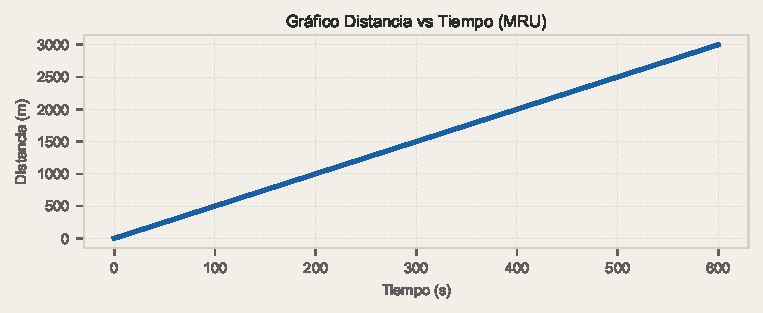
\includegraphics[width=12cm]{img_soluciones/vel_0.pdf}
\end{center}
\vspace{6pt}
\begin{tcolorbox}[colback=azul, colframe=azul, arc=4pt, boxrule=0.5pt,
  left=8pt, right=8pt, top=6pt, bottom=6pt, width=\textwidth]
  \textbf{\color{white} Problema 2: Tiempo de un corredor}
\end{tcolorbox}
\begin{tcolorbox}[colback=grisclr, colframe=gris, arc=4pt, boxrule=0.3pt,
  left=8pt, right=8pt, top=4pt, bottom=4pt, width=\textwidth]
  \small\textcolor{gris}{${v}$: 7 m/s (Norte)  $|$  ${d}$: 3 km = 3000 m}
\end{tcolorbox}
\hspace{12pt}$t = d / v$
\vspace{4pt}\textbf{\textcolor{teal}{Desarrollo:}}
\hspace{12pt}$t = 3000 / 7 = 428.57$ s
\hspace{12pt}En minutos: $428.57 / 60 = 7.14$ min
\vspace{4pt}
\resbox{Tiempo}{428.57 s (7.14 min)}
\begin{center}
  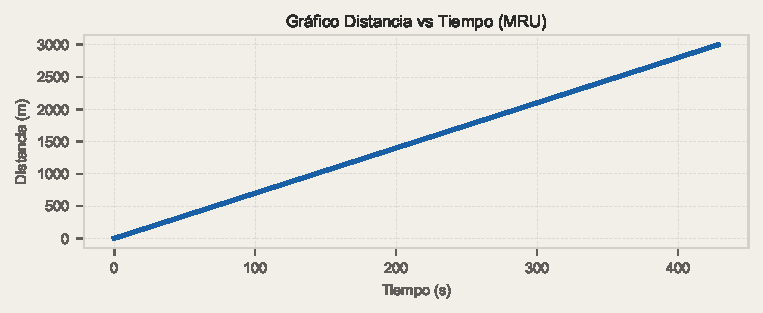
\includegraphics[width=12cm]{img_soluciones/vel_1.pdf}
\end{center}
\vspace{6pt}
\begin{tcolorbox}[colback=azul, colframe=azul, arc=4pt, boxrule=0.5pt,
  left=8pt, right=8pt, top=6pt, bottom=6pt, width=\textwidth]
  \textbf{\color{white} Problema 3: Distancia de una chita}
\end{tcolorbox}
\begin{tcolorbox}[colback=grisclr, colframe=gris, arc=4pt, boxrule=0.3pt,
  left=8pt, right=8pt, top=4pt, bottom=4pt, width=\textwidth]
  \small\textcolor{gris}{${v}$: 130 km/h  $|$  ${t}$: 4 min = 1/15 h}
\end{tcolorbox}
\hspace{12pt}$d = v \times t$
\vspace{4pt}\textbf{\textcolor{teal}{Desarrollo:}}
\hspace{12pt}$d = 130 \times 1/15 = 8.67$ km
\hspace{12pt}En metros: $8.67 \times 1000 = 8670$ m
\vspace{4pt}
\resbox{Distancia}{8.67 km (8670 m)}
\begin{center}
  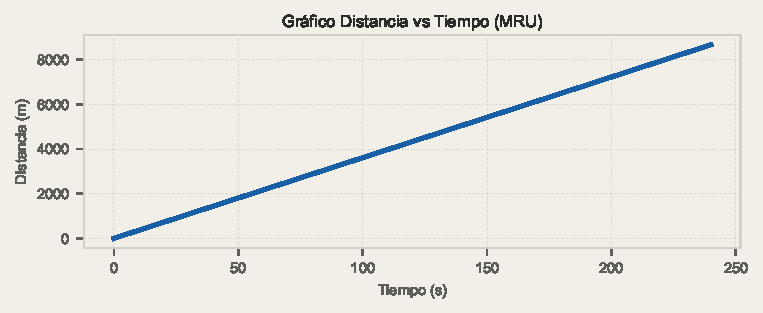
\includegraphics[width=12cm]{img_soluciones/vel_2.pdf}
\end{center}
\vspace{6pt}
\begin{tcolorbox}[colback=azul, colframe=azul, arc=4pt, boxrule=0.5pt,
  left=8pt, right=8pt, top=6pt, bottom=6pt, width=\textwidth]
  \textbf{\color{white} Problema 4: Velocidad de un bebé gateando}
\end{tcolorbox}
\begin{tcolorbox}[colback=grisclr, colframe=gris, arc=4pt, boxrule=0.3pt,
  left=8pt, right=8pt, top=4pt, bottom=4pt, width=\textwidth]
  \small\textcolor{gris}{${d}$: 8 m  $|$  ${t}$: 10 min = 600 s}
\end{tcolorbox}
\hspace{12pt}$v = d / t$
\vspace{4pt}\textbf{\textcolor{teal}{Desarrollo:}}
\hspace{12pt}$v = 8 / 600 = 0.0133$ m/s
\hspace{12pt}En km/h: $0.0133 \times 3.6 = 0.048$ km/h
\vspace{4pt}
\resbox{Velocidad}{0.0133 m/s (0.048 km/h)}
\begin{center}
  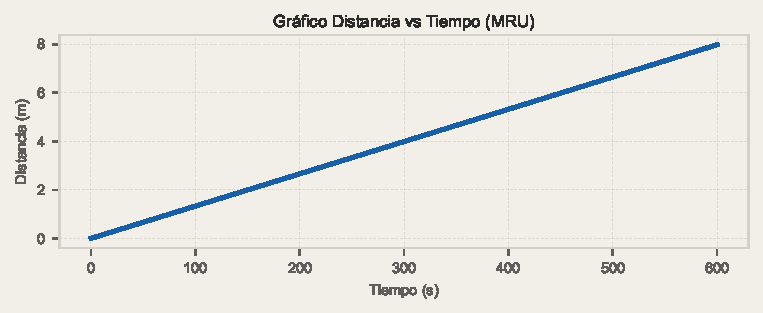
\includegraphics[width=12cm]{img_soluciones/vel_3.pdf}
\end{center}
\vspace{6pt}
\begin{tcolorbox}[colback=azul, colframe=azul, arc=4pt, boxrule=0.5pt,
  left=8pt, right=8pt, top=6pt, bottom=6pt, width=\textwidth]
  \textbf{\color{white} Problema 5: Distancia de un ciclista}
\end{tcolorbox}
\begin{tcolorbox}[colback=grisclr, colframe=gris, arc=4pt, boxrule=0.3pt,
  left=8pt, right=8pt, top=4pt, bottom=4pt, width=\textwidth]
  \small\textcolor{gris}{${v}$: 10 m/s  $|$  ${t}$: 125 s}
\end{tcolorbox}
\hspace{12pt}$d = v \times t$
\vspace{4pt}\textbf{\textcolor{teal}{Desarrollo:}}
\hspace{12pt}$d = 10 \times 125 = 1250$ m
\hspace{12pt}En km: $1250 / 1000 = 1.25$ km
\vspace{4pt}
\resbox{Distancia}{1250 m (1.25 km)}
\begin{center}
  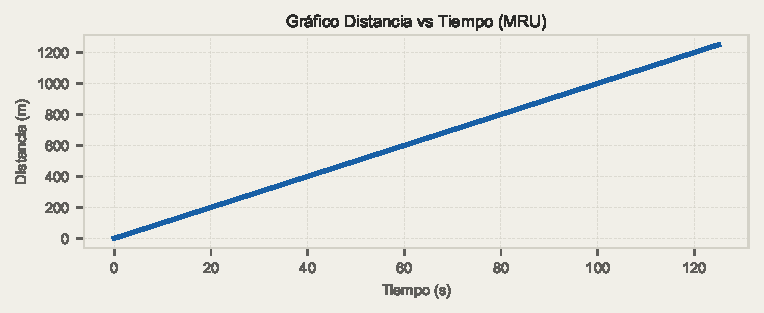
\includegraphics[width=12cm]{img_soluciones/vel_4.pdf}
\end{center}
\vspace{6pt}
\begin{tcolorbox}[colback=azul, colframe=azul, arc=4pt, boxrule=0.5pt,
  left=8pt, right=8pt, top=6pt, bottom=6pt, width=\textwidth]
  \textbf{\color{white} Problema 6: Velocidad de un motociclista}
\end{tcolorbox}
\begin{tcolorbox}[colback=grisclr, colframe=gris, arc=4pt, boxrule=0.3pt,
  left=8pt, right=8pt, top=4pt, bottom=4pt, width=\textwidth]
  \small\textcolor{gris}{${d}$: 8 km = 8000 m (Este)  $|$  ${t}$: 9 min = 540 s}
\end{tcolorbox}
\hspace{12pt}$v = d / t$
\vspace{4pt}\textbf{\textcolor{teal}{Desarrollo:}}
\hspace{12pt}$v = 8000 / 540 = 14.81$ m/s
\vspace{4pt}
\resbox{Velocidad}{14.81 m/s hacia el Este}
\begin{center}
  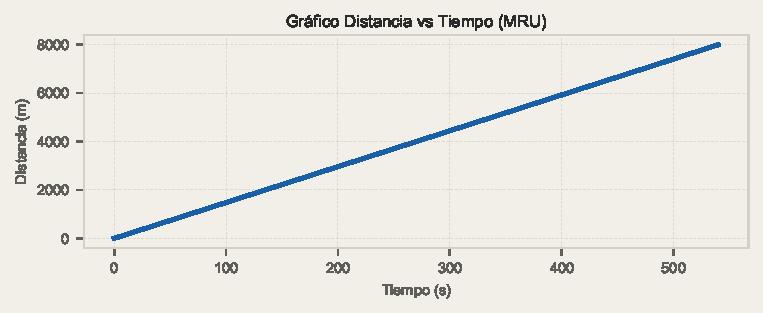
\includegraphics[width=12cm]{img_soluciones/vel_5.pdf}
\end{center}
\vspace{6pt}
\begin{tcolorbox}[colback=azul, colframe=azul, arc=4pt, boxrule=0.5pt,
  left=8pt, right=8pt, top=6pt, bottom=6pt, width=\textwidth]
  \textbf{\color{white} Problema 7: Desplazamiento de un automóvil}
\end{tcolorbox}
\begin{tcolorbox}[colback=grisclr, colframe=gris, arc=4pt, boxrule=0.3pt,
  left=8pt, right=8pt, top=4pt, bottom=4pt, width=\textwidth]
  \small\textcolor{gris}{${v}$: 80 km/h (Norte)  $|$  ${t}$: 0.8 min = 48 s}
\end{tcolorbox}
\hspace{12pt}$d = v \times t$
\vspace{4pt}\textbf{\textcolor{teal}{Desarrollo:}}
\hspace{12pt}$v = 80 / 3.6 = 22.22$ m/s
\hspace{12pt}$d = 22.22 \times 48 = 1067$ m
\vspace{4pt}
\resbox{Desplazamiento}{1067 m hacia el Norte}
\begin{center}
  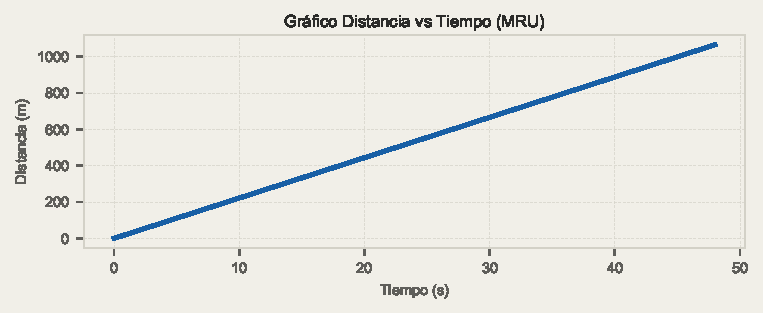
\includegraphics[width=12cm]{img_soluciones/vel_6.pdf}
\end{center}
\vspace{6pt}
\hrule height 0.5pt\vspace{10pt}
\section{Ejercicios de Aceleración}
\begin{tcolorbox}[colback=coral, colframe=coral, arc=4pt, boxrule=0.5pt,
  left=8pt, right=8pt, top=6pt, bottom=6pt, width=\textwidth]
  \textbf{\color{white} Problema 1: Avión aterrizando en portaaviones}
\end{tcolorbox}
\begin{tcolorbox}[colback=grisclr, colframe=gris, arc=4pt, boxrule=0.3pt,
  left=8pt, right=8pt, top=4pt, bottom=4pt, width=\textwidth]
  \small\textcolor{gris}{$$V_i$$: 90 m/s  $|$  $$V_f$$: 0 m/s  $|$  $$d$$: 100 m}
\end{tcolorbox}
\hspace{12pt}$V_f^2 = V_i^2 + 2ad$
\hspace{12pt}$V_f = V_i + at$
\vspace{4pt}\textbf{\textcolor{teal}{Desarrollo:}}
\hspace{12pt}a) Aceleración: $0^2 = 90^2 + 2a(100) \to a = -8100/200 = -40.5$ m/s$^2$
\hspace{12pt}b) Tiempo: $0 = 90 + (-40.5)t \to t = 90/40.5 = 2.22$ s
\vspace{4pt}
\resbox{Aceleración}{$-40.5$ m/s$^2$ (desaceleración)}
\resbox{Tiempo}{2.22 s}
\begin{center}
  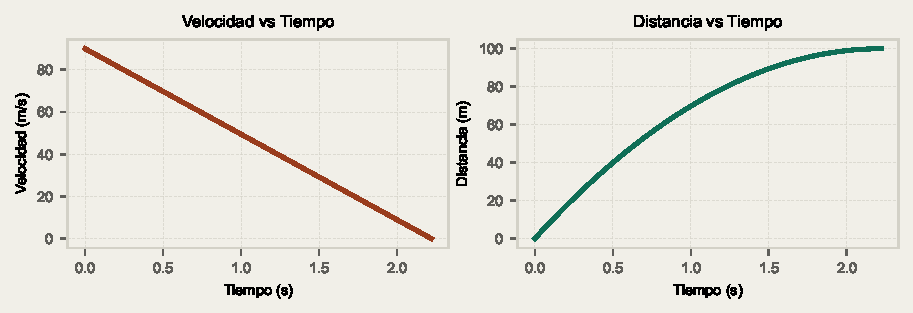
\includegraphics[width=14cm]{img_soluciones/acel_0.pdf}
\end{center}
\vspace{6pt}
\begin{tcolorbox}[colback=coral, colframe=coral, arc=4pt, boxrule=0.5pt,
  left=8pt, right=8pt, top=6pt, bottom=6pt, width=\textwidth]
  \textbf{\color{white} Problema 2: Tren acelerando constantemente}
\end{tcolorbox}
\begin{tcolorbox}[colback=grisclr, colframe=gris, arc=4pt, boxrule=0.3pt,
  left=8pt, right=8pt, top=4pt, bottom=4pt, width=\textwidth]
  \small\textcolor{gris}{$$V_i$$: 16 m/s  $|$  $$a$$: 2 m/s$^2$  $|$  $$t$$: 20 s}
\end{tcolorbox}
\hspace{12pt}$d = V_i t + \frac{1}{2} a t^2$
\hspace{12pt}$V_f = V_i + at$
\vspace{4pt}\textbf{\textcolor{teal}{Desarrollo:}}
\hspace{12pt}a) Distancia: $d = 16(20) + \frac{1}{2}(2)(20)^2 = 320 + 400 = 720$ m
\hspace{12pt}b) Velocidad final: $V_f = 16 + 2(20) = 56$ m/s
\vspace{4pt}
\resbox{Distancia}{720 m}
\resbox{Velocidad final}{56 m/s}
\begin{center}
  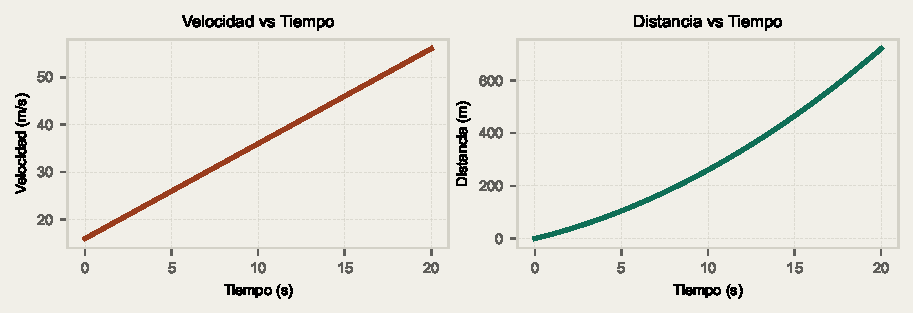
\includegraphics[width=14cm]{img_soluciones/acel_1.pdf}
\end{center}
\vspace{6pt}
\begin{tcolorbox}[colback=coral, colframe=coral, arc=4pt, boxrule=0.5pt,
  left=8pt, right=8pt, top=6pt, bottom=6pt, width=\textwidth]
  \textbf{\color{white} Problema 3: Lancha de motor desde el reposo}
\end{tcolorbox}
\begin{tcolorbox}[colback=grisclr, colframe=gris, arc=4pt, boxrule=0.3pt,
  left=8pt, right=8pt, top=4pt, bottom=4pt, width=\textwidth]
  \small\textcolor{gris}{$$V_i$$: 0 m/s  $|$  $$V_f$$: 15 m/s  $|$  $$t$$: 6 s}
\end{tcolorbox}
\hspace{12pt}$a = (V_f - V_i) / t$
\hspace{12pt}$d = V_i t + \frac{1}{2} a t^2$
\vspace{4pt}\textbf{\textcolor{teal}{Desarrollo:}}
\hspace{12pt}a) Aceleración: $a = (15 - 0)/6 = 2.5$ m/s$^2$
\hspace{12pt}b) Distancia: $d = 0 + \frac{1}{2}(2.5)(6)^2 = 1.25 \times 36 = 45$ m
\vspace{4pt}
\resbox{Aceleración}{2.5 m/s$^2$}
\resbox{Distancia}{45 m}
\begin{center}
  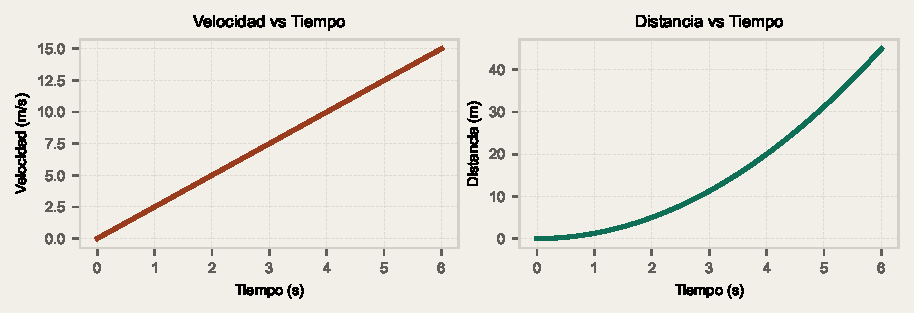
\includegraphics[width=14cm]{img_soluciones/acel_2.pdf}
\end{center}
\vspace{6pt}
\begin{tcolorbox}[colback=coral, colframe=coral, arc=4pt, boxrule=0.5pt,
  left=8pt, right=8pt, top=6pt, bottom=6pt, width=\textwidth]
  \textbf{\color{white} Problema 4: Automóvil de carreras}
\end{tcolorbox}
\begin{tcolorbox}[colback=grisclr, colframe=gris, arc=4pt, boxrule=0.3pt,
  left=8pt, right=8pt, top=4pt, bottom=4pt, width=\textwidth]
  \small\textcolor{gris}{$$V_i$$: 20 m/s  $|$  $$V_f$$: 37 m/s  $|$  $$t$$: 2.5 s}
\end{tcolorbox}
\hspace{12pt}$a = (V_f - V_i) / t$
\vspace{4pt}\textbf{\textcolor{teal}{Desarrollo:}}
\hspace{12pt}$a = (37 - 20) / 2.5 = 17 / 2.5 = 6.8$ m/s$^2$
\vspace{4pt}
\resbox{Aceleración}{6.8 m/s$^2$}
\begin{center}
  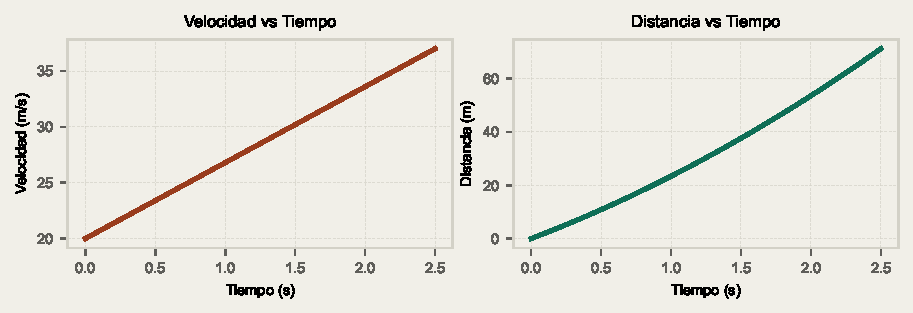
\includegraphics[width=14cm]{img_soluciones/acel_3.pdf}
\end{center}
\vspace{6pt}
\begin{tcolorbox}[colback=coral, colframe=coral, arc=4pt, boxrule=0.5pt,
  left=8pt, right=8pt, top=6pt, bottom=6pt, width=\textwidth]
  \textbf{\color{white} Problema 5: Motociclista frenando}
\end{tcolorbox}
\begin{tcolorbox}[colback=grisclr, colframe=gris, arc=4pt, boxrule=0.3pt,
  left=8pt, right=8pt, top=4pt, bottom=4pt, width=\textwidth]
  \small\textcolor{gris}{$$V_i$$: 35 m/s  $|$  $$V_f$$: 0 m/s  $|$  $$t$$: 1.8 s}
\end{tcolorbox}
\hspace{12pt}$a = (V_f - V_i) / t$
\vspace{4pt}\textbf{\textcolor{teal}{Desarrollo:}}
\hspace{12pt}$a = (0 - 35) / 1.8 = -35 / 1.8 = -19.44$ m/s$^2$
\vspace{4pt}
\resbox{Desaceleración}{$-19.44$ m/s$^2$}
\begin{center}
  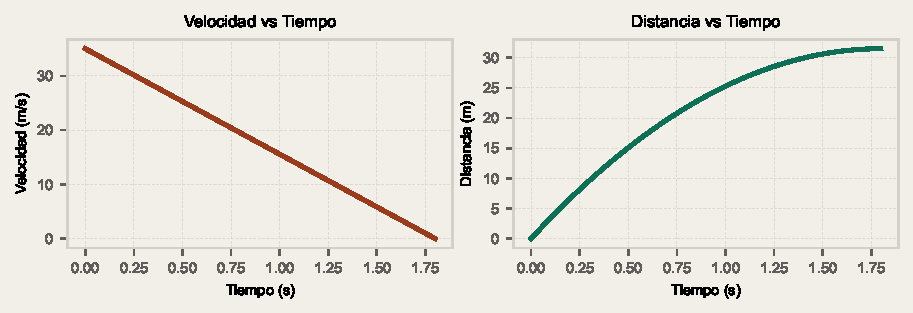
\includegraphics[width=14cm]{img_soluciones/acel_4.pdf}
\end{center}
\vspace{6pt}
\begin{tcolorbox}[colback=coral, colframe=coral, arc=4pt, boxrule=0.5pt,
  left=8pt, right=8pt, top=6pt, bottom=6pt, width=\textwidth]
  \textbf{\color{white} Problema 6: Automóvil de carreras (2)}
\end{tcolorbox}
\begin{tcolorbox}[colback=grisclr, colframe=gris, arc=4pt, boxrule=0.3pt,
  left=8pt, right=8pt, top=4pt, bottom=4pt, width=\textwidth]
  \small\textcolor{gris}{$$V_i$$: 18.5 m/s  $|$  $$V_f$$: 46.1 m/s  $|$  $$t$$: 2.47 s}
\end{tcolorbox}
\hspace{12pt}$a = (V_f - V_i) / t$
\vspace{4pt}\textbf{\textcolor{teal}{Desarrollo:}}
\hspace{12pt}$a = (46.1 - 18.5) / 2.47 = 27.6 / 2.47 = 11.17$ m/s$^2$
\vspace{4pt}
\resbox{Aceleración}{11.17 m/s$^2$}
\begin{center}
  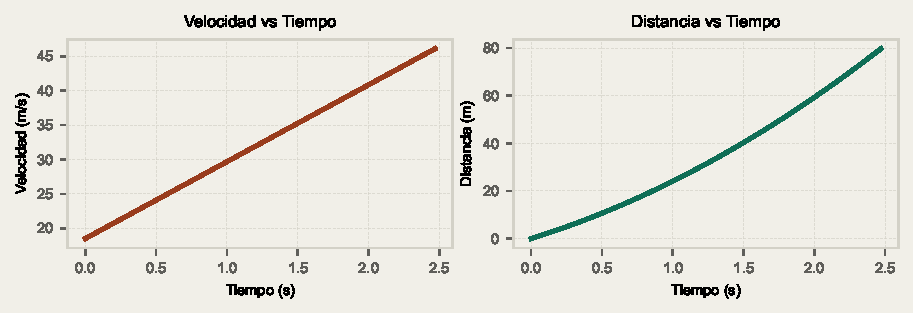
\includegraphics[width=14cm]{img_soluciones/acel_5.pdf}
\end{center}
\vspace{6pt}
\begin{tcolorbox}[colback=coral, colframe=coral, arc=4pt, boxrule=0.5pt,
  left=8pt, right=8pt, top=6pt, bottom=6pt, width=\textwidth]
  \textbf{\color{white} Problema 7: Motociclista frenando (2)}
\end{tcolorbox}
\begin{tcolorbox}[colback=grisclr, colframe=gris, arc=4pt, boxrule=0.3pt,
  left=8pt, right=8pt, top=4pt, bottom=4pt, width=\textwidth]
  \small\textcolor{gris}{$$V_i$$: 22.4 m/s  $|$  $$V_f$$: 0 m/s  $|$  $$t$$: 2.55 s}
\end{tcolorbox}
\hspace{12pt}$a = (V_f - V_i) / t$
\vspace{4pt}\textbf{\textcolor{teal}{Desarrollo:}}
\hspace{12pt}$a = (0 - 22.4) / 2.55 = -22.4 / 2.55 = -8.78$ m/s$^2$
\vspace{4pt}
\resbox{Desaceleración}{$-8.78$ m/s$^2$}
\begin{center}
  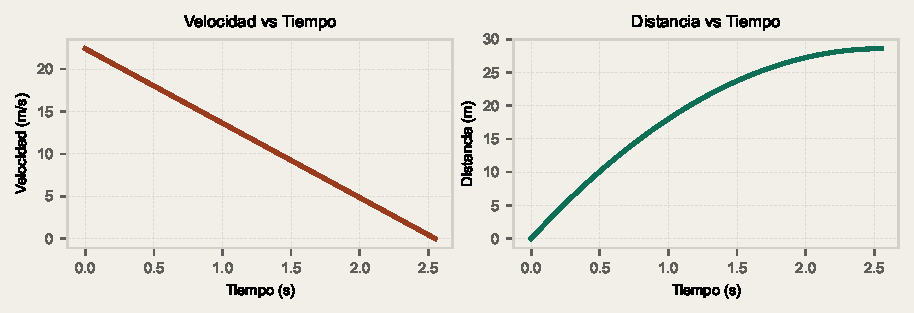
\includegraphics[width=14cm]{img_soluciones/acel_6.pdf}
\end{center}
\vspace{6pt}
\begin{tcolorbox}[colback=coral, colframe=coral, arc=4pt, boxrule=0.5pt,
  left=8pt, right=8pt, top=6pt, bottom=6pt, width=\textwidth]
  \textbf{\color{white} Problema 8: Camión de bomberos}
\end{tcolorbox}
\begin{tcolorbox}[colback=grisclr, colframe=gris, arc=4pt, boxrule=0.3pt,
  left=8pt, right=8pt, top=4pt, bottom=4pt, width=\textwidth]
  \small\textcolor{gris}{$$V_i$$: 0 m/s  $|$  $$V_f$$: 21 m/s (Este)  $|$  $$t$$: 3.5 s}
\end{tcolorbox}
\hspace{12pt}$a = (V_f - V_i) / t$
\vspace{4pt}\textbf{\textcolor{teal}{Desarrollo:}}
\hspace{12pt}$a = (21 - 0) / 3.5 = 6$ m/s$^2$
\vspace{4pt}
\resbox{Aceleración}{6 m/s$^2$ hacia el Este}
\begin{center}
  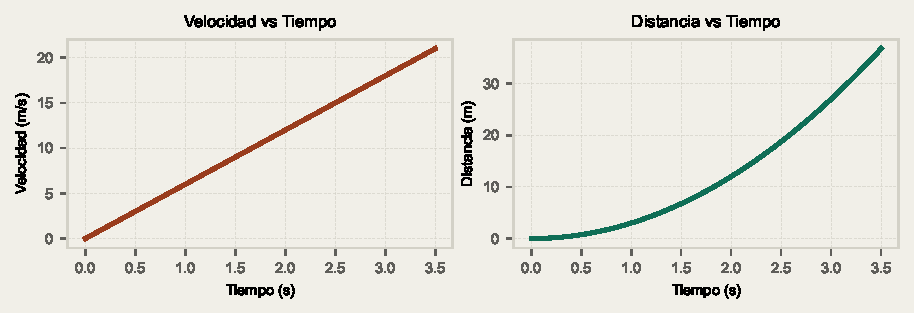
\includegraphics[width=14cm]{img_soluciones/acel_7.pdf}
\end{center}
\vspace{6pt}
\begin{tcolorbox}[colback=coral, colframe=coral, arc=4pt, boxrule=0.5pt,
  left=8pt, right=8pt, top=6pt, bottom=6pt, width=\textwidth]
  \textbf{\color{white} Problema 9: Automóvil en autopista}
\end{tcolorbox}
\begin{tcolorbox}[colback=grisclr, colframe=gris, arc=4pt, boxrule=0.3pt,
  left=8pt, right=8pt, top=4pt, bottom=4pt, width=\textwidth]
  \small\textcolor{gris}{$$V_i$$: 80 km/h = 22.22 m/s  $|$  $$V_f$$: 110 km/h = 30.56 m/s  $|$  $$a$$: 1.8 m/s$^2$}
\end{tcolorbox}
\hspace{12pt}$t = (V_f - V_i) / a$
\vspace{4pt}\textbf{\textcolor{teal}{Desarrollo:}}
\hspace{12pt}$t = (30.56 - 22.22) / 1.8 = 8.34 / 1.8 = 4.63$ s
\vspace{4pt}
\resbox{Tiempo}{4.63 s}
\begin{center}
  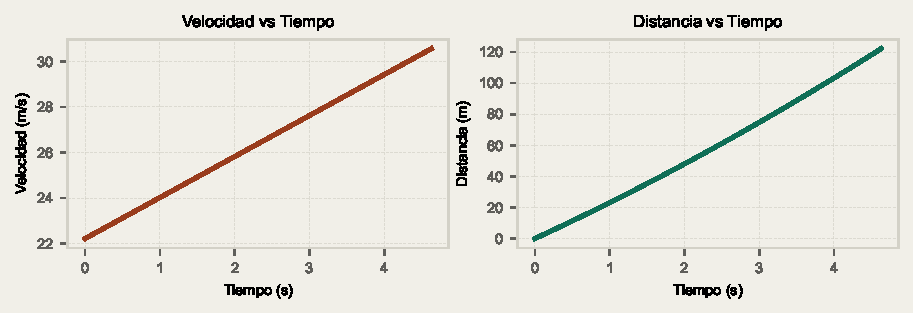
\includegraphics[width=14cm]{img_soluciones/acel_8.pdf}
\end{center}
\vspace{6pt}
\hrule height 0.5pt\vspace{10pt}
\section{Resumen de Resultados}
\begin{tabularx}{\textwidth}{LC}
  \toprule\rowcolor{teal}
  \textbf{\textcolor{white}{Ejercicio}} & \textbf{\textcolor{white}{Resultado Principal}} \\
  \midrule
  Velocidad 1 & 18 km/h (5 m/s) \\
  \rowcolor{tealclr}
  Velocidad 2 & 428.57 s (7.14 min) \\
  Velocidad 3 & 8.67 km (8670 m) \\
  \rowcolor{tealclr}
  Velocidad 4 & 0.0133 m/s \\
  Velocidad 5 & 1250 m \\
  \rowcolor{tealclr}
  Velocidad 6 & 14.81 m/s al Este \\
  Velocidad 7 & 1067 m al Norte \\
  \rowcolor{tealclr}
  Aceleración 1 & $a = -40.5$ m/s$^2$, $t = 2.22$ s \\
  Aceleración 2 & $d = 720$ m, $V_f = 56$ m/s \\
  \rowcolor{tealclr}
  Aceleración 3 & $a = 2.5$ m/s$^2$, $d = 45$ m \\
  Aceleración 4 & $a = 6.8$ m/s$^2$ \\
  \rowcolor{tealclr}
  Aceleración 5 & $a = -19.44$ m/s$^2$ \\
  Aceleración 6 & $a = 11.17$ m/s$^2$ \\
  \rowcolor{tealclr}
  Aceleración 7 & $a = -8.78$ m/s$^2$ \\
  Aceleración 8 & $a = 6$ m/s$^2$ al Este \\
  \rowcolor{tealclr}
  Aceleración 9 & $t = 4.63$ s \\
  \bottomrule
\end{tabularx}
\vspace{8pt}
\begin{tcolorbox}[colback=grisclr, colframe=gris, arc=4pt, boxrule=0.3pt,
  left=8pt, right=8pt, top=4pt, bottom=4pt, width=\textwidth]
  \small\textcolor{gris}{Nota: Todos los cálculos utilizan el Sistema Internacional de Unidades (SI).}
  \small\textcolor{gris}{Las desaceleraciones se representan con signo negativo.}
\end{tcolorbox}
\end{document}